\chapter{背景知识}
本章主要对本文所涉及的支持向量机、关系图卷积神经网络、双向长短期记忆神经网络、注意力机制等展开了详细的描述,为下文第三章、第四章和第五章的内容做好铺垫。

在构建组件-事件知识图谱时,第三章通过实验分析最终选用了支持向量机发掘事件因果关系,因此本章第一节对支持向量机进行了介绍。第四章组件-事件知识图谱表示学习是基于关系图卷积神经网络提出的,为了便于理解这部分内容,本章第二节对关系图卷积神经网络进行了必要地介绍。第五章基于知识图谱的故障预测是基于双向长短期记忆网络提出的,所以本章第三节对双向长短期记忆网络展开介绍。另外,第四章和第五章所提出的方法,都引入了注意力机制,所以本章第四节又介绍了注意力机制。

\section{支持向量机}
支持向量机(Support Vector Machines,SVM)是机器学习和模式分类领域的经典模型\cite{cherkassky2004practical},通过在输入空间中实现线性或非线性分离面来实现分类。在支持向量分类中,分离函数可以表示为与支持向量相关的核的线性组合,如式\ref{bk-svm}所示:
\begin{equation}
    \centering
    f(x)=\sum_{x_{j} \in S} \alpha_{j} y_{j} K\left(x_{j}, x\right)+b
    \label{bk-svm}
\end{equation}
其中$x_{i}$表示训练模式,$y_{i} \in\{+1,-1\}$表示相应的类标签,$S$表示支持向量集\cite{cherkassky2004practical}。其对偶式如式子\ref{bk-svm-op}所示:
\begin{equation}
    \centering
    \min _{0 \leq \alpha_{i} \leq C} W=\frac{1}{2} \sum_{i, j} \alpha_{i} Q_{i j} \alpha_{j}-\sum_{i} \alpha_{i}+b \sum_{i} y_{i} \alpha_{i}
    \label{bk-svm-op}
\end{equation}
其中$\alpha_{i}$是相应的协同系数,$b$是偏移系数,$Q_{i j}=y_{i} y_{j} K\left(x_{i}, x_{j}\right)$是一个对称的正定核矩阵,$C$是在不可分的情况下用来惩罚误差点的参数\cite{cherkassky2004practical}。对偶的Karush-Kuhn-Tucker(KKT)条件如式\ref{bk-svm-KKT}和式\ref{bk-svm-KKT-2}所示:
\begin{equation}
    \centering
    g_{i}=\frac{\partial W}{\partial \alpha_{i}}=\sum_{i} Q_{i j} \alpha_{j}+y_{i} b-1=y_{i} f\left(x_{i}\right)-1
    \label{bk-svm-KKT}
\end{equation}
\begin{equation}
    \centering
    \frac{\partial W}{\partial b}=\sum_{j} y_{j} \alpha_{j}=0
    \label{bk-svm-KKT-2}
\end{equation}

其将训练集划分为支持向量集$S$$\left(0<\alpha_{i}<C, g_{i}=0\right)$,误差集$E$$\left(\alpha_{i}=C, g_{i}<0\right)$和分类集$R$$\left(\alpha_{i}=0, g_{i}>0\right)$\cite{cauwenberghs2001incremental}。如果误差点用惩罚因子$C^{\prime}$进行二次罚分,那么这表明问题已经被简化为$C=\infty$的可分情形\cite{frie1998kernel}。内核函数可以修改为式\ref{bk-svm-modekernel}所示。
\begin{equation}
    \centering
    K^{\prime}\left(x_{i}, x_{j}\right)=K\left(x_{i}, x_{j}\right)+\frac{1}{C^{\prime}} \delta_{i j}
    \label{bk-svm-modekernel}
\end{equation}

其中当$i=j$时$\delta_{i j}=1$,否则$\delta_{i j}=0$。这个公式的优点是SVM问题可以被简化为线性可分情形\cite{keerthi2000fast}。

由上可见,训练SVM时要解一个二次优化问题,这需要使用来自数值库的优化例程。另外,解二次优化问题是计算密集型的,可能会遇到稳定性问题,并且实现起来非常困难\cite{zeng2008fast}。因此,序列最小优化(Sequential Minimal Optimization,SMO)\cite{keerthi2000fast}和最近点算法(NearestPoint Algorithm ,NPA)\cite{zeng2008fast},相继被提出并成功克服了这个问题。


\section{关系图卷积神经网络}\label{RGCN}
本小节主要介绍关系图卷积神经网络(Relational Graph Convolutional Networks,RGCN)算法\cite{schlichtkrull2018modeling}。该算法区分了不同关系对节点的影响,利用图信息传播机制获取了实体的上下文信息。本节会进一步分为两小节分别介绍RGCN的模型结构和优化目标。
% 下一小节中,本文在此模型基础上考虑了图信息传播时同一关系下不同实体的权重。
\subsection{模型结构}
本小节介绍RGCN的模型结构,包括嵌入层和图卷积层。

嵌入层主要为了引入实体多维度的信息,如实体包含着的各种语义信息。对于每个实体,该文献将其不同的文本属性连接起来,并使用预先训练的Bert\cite{devlin2018bert}模型来获得它们的嵌入表示。这些嵌入表示形成了实体的初始特征向量。对于实体没有属性的数据集,嵌入层则是随机初始化的。

图卷积层使用图卷积网络将局部的信息通过关系传递到整个图中,因此可以将其理解为一个可微分的消息传递框架,可以用式子\ref{propo-example}表示。
\begin{equation}
    h_{i}^{(l+1)}=\sigma\left(\sum_{m \in \mathcal{M}_{i}} g_{m}\left(h_{i}^{(l)}, h_{j}^{(l)}\right)\right)
    \label{propo-example}
\end{equation}

$h_{i}^{(l)} \in \mathbb{R}^{d^{(l)}}$是结点$v_{i}$在$l$-th层神经网络的隐状态,$d^{(l)}$是该层隐状态向量的维度。$g_{m}(\cdot, \cdot)$函数计算了$v_{j}$传入结点$v_{i}$的信息。随后累加$v_{i}$每个邻居结点传来的信息,并将累计结果传入激活函数$\sigma(\cdot)$就可以得到$v_{i}$在下一层神经网络的隐状态向量$h_{i}^{(l+1)}$,其中激活函数可以使用$\operatorname{ReLU}(\cdot)=\max (0, \cdot)$等常见的激活函数。$\mathcal{M}_{i}$表示每一条传入结点$v_{i}$的信息汇总集,其中每一条传入信息都与一条边对应。$g_{m}(\cdot, \cdot)$通常为信息计算函数,具体实现上可以是某种神经网络也可以是某种线性转变,比如$g_{m}\left(h_{i}, h_{j}\right)=W h_{j}$,$W$为参数张量(如文献\parencite{kipf2016semi}所示)。这样的信息计算函数有效地累计并编码了来自局部的结构化邻域特征,并在诸如图分类\cite{duvenaud2015convolutional}和图的半监督学习等领域取得了显著的改进效果。

基于上文的消息传递架构,一个知识图谱可以表示为$Graph=\left(\mathcal{V},\mathcal{E},\mathcal{R}\right)$,其中$v_i\in\mathcal{V}$表示结点,$\left(v_i,r,v_j\right)\in\mathcal{E}$表示被标注的边,$r\in\mathcal{R}$表示关系类型。
% 在本文中,$\mathcal{R}$包含正向因果(导致)、反向因果(被导致)两种关系类型。
其信息传播过程如式\ref{propo-in-directedgraph}所示。该式用于计算有向图中由$v_{i}$表示的实体或节点的隐状态随信息传递的变化。
\begin{equation}
    h_{i}^{(l+1)}=\sigma\left(\sum_{r \in \mathcal{R}} \sum_{j \in \mathcal{N}_{i}^{r}} \frac{1}{c_{i, r}} W_{r}^{(l)} h_{j}^{(l)}+W_{0}^{(l)} h_{i}^{(l)}\right)
    \label{propo-in-directedgraph}
\end{equation}
其中,$h_i^{\left(l\right)}\in R^{d^{\left(l\right)}}$为结点$v_i$在第$l$层神经网络的隐状态,$d^{\left(l\right)}$是该层网络表示空间的维度。而$\mathcal{N}_{i}^{r}$是索引为i的结点在关系$r\in\mathcal{R}$下的所有邻接结点索引值集合。$c_{i,r}$是特定于问题的规范化常量,可以被学习或预先指定(例如$c_{i, r}=\left|\mathcal{N}_{i}^{r}\right|$)。该方法通过归一化和来计算相邻节点传播来的信息,并且只选择相邻结点进行线性变换$Wh_j$具有重要的计算优势,既不需要使用大量内存保存关系向量,也可以通过使用稀疏矩阵乘法减少资源消耗。

\begin{figure}[htbp]
    \centering
    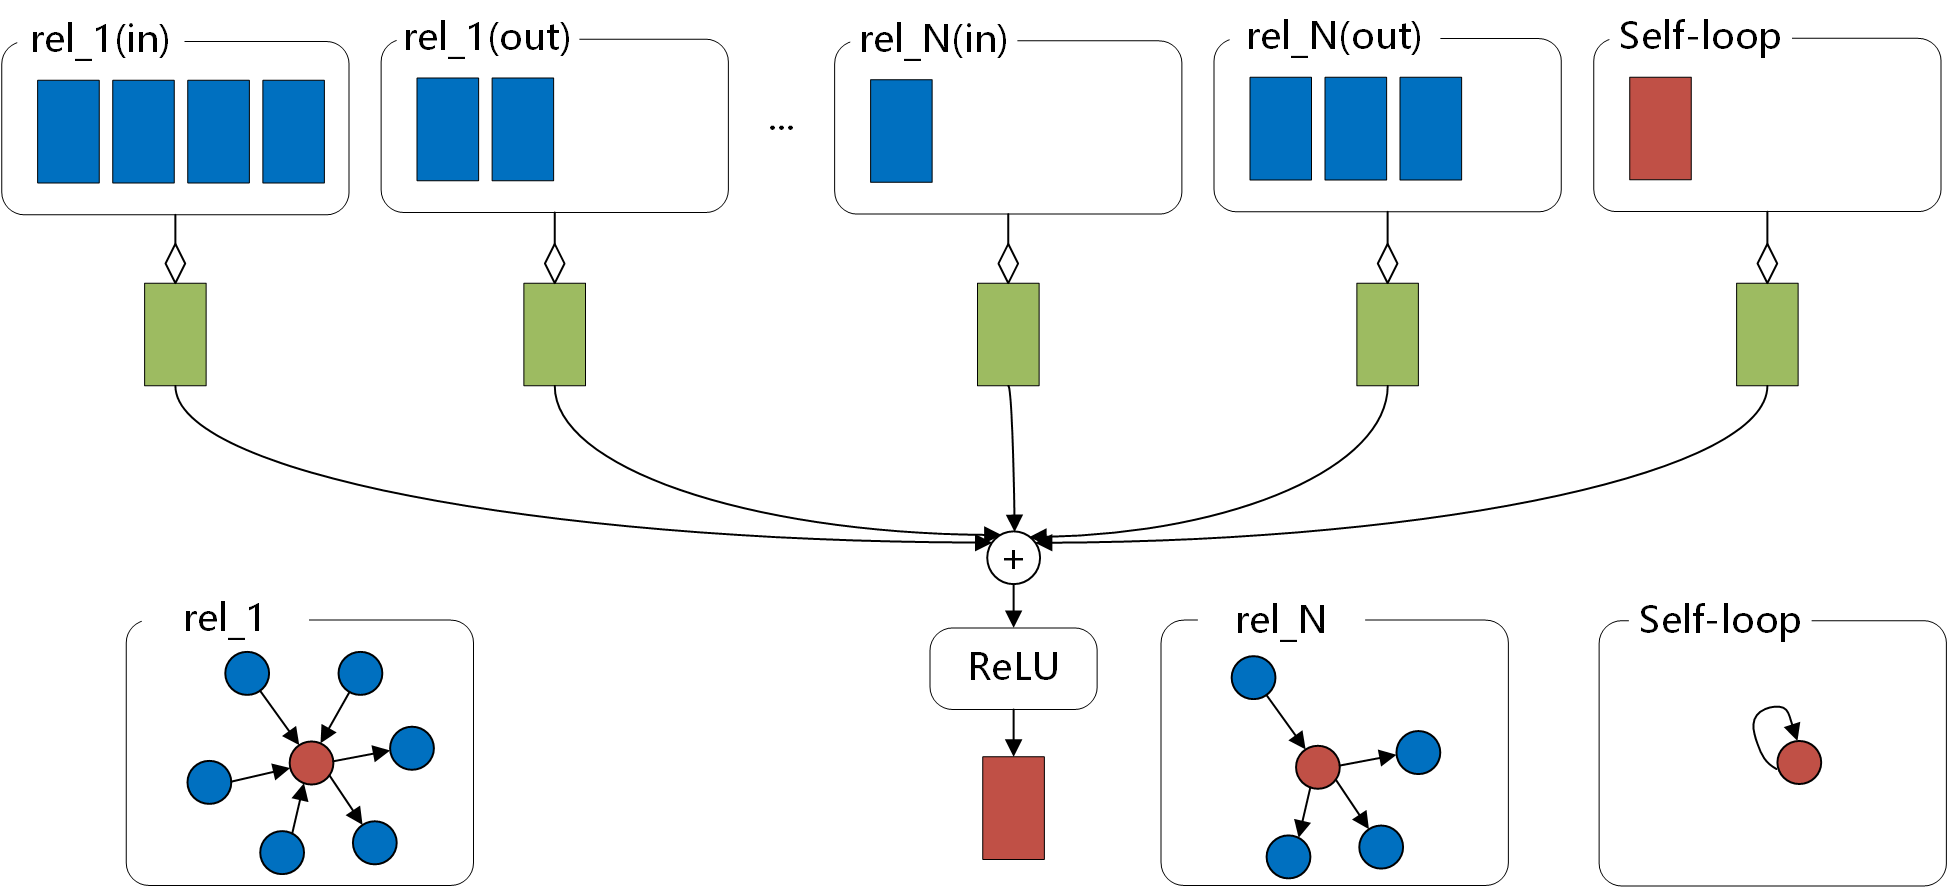
\includegraphics[width=.8\textwidth]{rgcn-cal.png}
    \caption{每层图网络隐状态更新过程\label{rgcn-cal}}
\end{figure}

每一层图网络的更新都需要对有向图中每个节点按照公式\ref{propo-in-directedgraph}进行并行计算。在模型实现中,可以堆叠多个图网络层以获取跨多个边的依赖关系。其中单个节点更新的计算图如图\ref{rgcn-cal}所示。待更新隐状态的结点或实体为红色,其所有的一跳邻居结点都为蓝色,用$d$维度的向量表示。然后针对每个relation类型分别进行信息传播计算,信息计算结果表示以标准化和的形式累加(绿色),最后经过激活函数作为新的隐状态向量,激活函数可以选择ReLU等。

\subsection{优化目标}
模型在进行参数更新时,主要使用了来自实体分类和链接预测两方面的损失函数。

实体分类:将如式子\ref{propo-in-directedgraph}的每一层图神经网络堆叠起来,并在最后一层节点的输出隐状态向量上使用$\operatorname{softmax}(\cdot)$激活函数。最终在标注的结点上最小化式\ref{node-class-crossenphory}表示的交叉熵损失函数即可。
\begin{equation}
    \mathcal{L}=-\sum_{i \in \mathcal{Y}} \sum_{k=1}^{K} t_{i k} \ln h_{i k}^{(L)}
    \label{node-class-crossenphory}
\end{equation}

其中$\mathcal{Y}$是有标签的结点索引集,$h_{i k}^{(L)}$是索引为$i$的带标签结点对应的网络输出的第$k$维的实数值。$t_{i k}$表示该实体的标注向量第$k$维的实数值。最后使用梯度下降算法训练模型参数即可。

链接预测:预测事实存在还是不存在(即三元组$(head,relation,tail)$是否存在)。有向、有标注的知识图谱可以使用符号式表示,即$G=(\mathcal{V}, \mathcal{E}, \mathcal{R})$。训练过程中没有使用完整的边集$\mathcal{E}$,而是使用了其子集$\hat{\mathcal{E}}$。模型会给候选边$(h, r, t)$一个分数$f(h, r, t)$,用以确定该边属于$\mathcal{E}$的可能性有多大。
为了进行链接预测,该文献引入了图编码-解码模型,编码部分使用上述图神经网络编码实体,解码部分对应着一个打分函数。编码器将每一个实体$v_{i} \in \mathcal{V}$映射到一个实数向量$e_{i} \in \mathbb{R}^{d}$。解码器会根据编码器输出的实体表示预测链接,具体实现上就是通过形如$s: \mathbb{R}^{d} \times \mathcal{R} \times \mathbb{R}^{d} \rightarrow \mathbb{R}$的函数给三元组$(head, relation, tail)$评分。编码器选用了上述的图卷积网络,解码器选用了文献\parencite{yang2014embedding}中的DistMult模型。DistMult模型中每一个关系$r$都与对角矩阵$R_{r} \in \mathbb{R}^{d \times d}$相关,候选三元组可以用式\ref{rgcn-link-score}计算得到评分。
\begin{equation}
    f(h, r, t)=e_{h}^{T} R_{r} e_{t}
    \label{rgcn-link-score}
\end{equation}
训练时,使用负采样为每个三元组负采样$\omega$个负样本。负样本来自于将正确的三元组的head或tail随机地替换掉。最终以正确的三元组评分要高于负样本为目的,使用了以下式\ref{rgcn-link-loss}为损失函数。

\begin{equation}
    \begin{aligned}
        \mathcal{L}=-\frac{1}{(1+\omega)|\hat{\mathcal{E}}|} & \sum_{(h, r, t, y) \in \mathcal{T}} y \log l(f(h, r, t))+\\
        &(1-y) \log (1-l(f(h, r, t)))
        \end{aligned}
    \label{rgcn-link-loss}
\end{equation}
其中$\mathcal{T}$是包含了正确和错误三元组的集合,而$l$是sigmoid函数。$y$是三元组的标签,$y=1$表示该三元组是正确的,$y=0$表示该三元组是错误的。在计算得到损失值后,会使用随机梯度下降算法更新模型参数。

\section{双向长短期记忆神经网络}\label{memory-net-section}
本节主要介绍编码时序数据的双向长短期记忆神经网络(Bi-directional Long Short-Term Memory,BiLSTM)。双向长短期记忆神经网络被广泛运用在许多场景中,本文以文献\parencite{gao2020task}中使用该模型进行故障预测为例,展开具体介绍。本节会进一步分为两小节分别介绍 BiLSTM 的模型结构和优化目标。
\subsection{模型结构}
\begin{figure}[htbp]
    \centering
    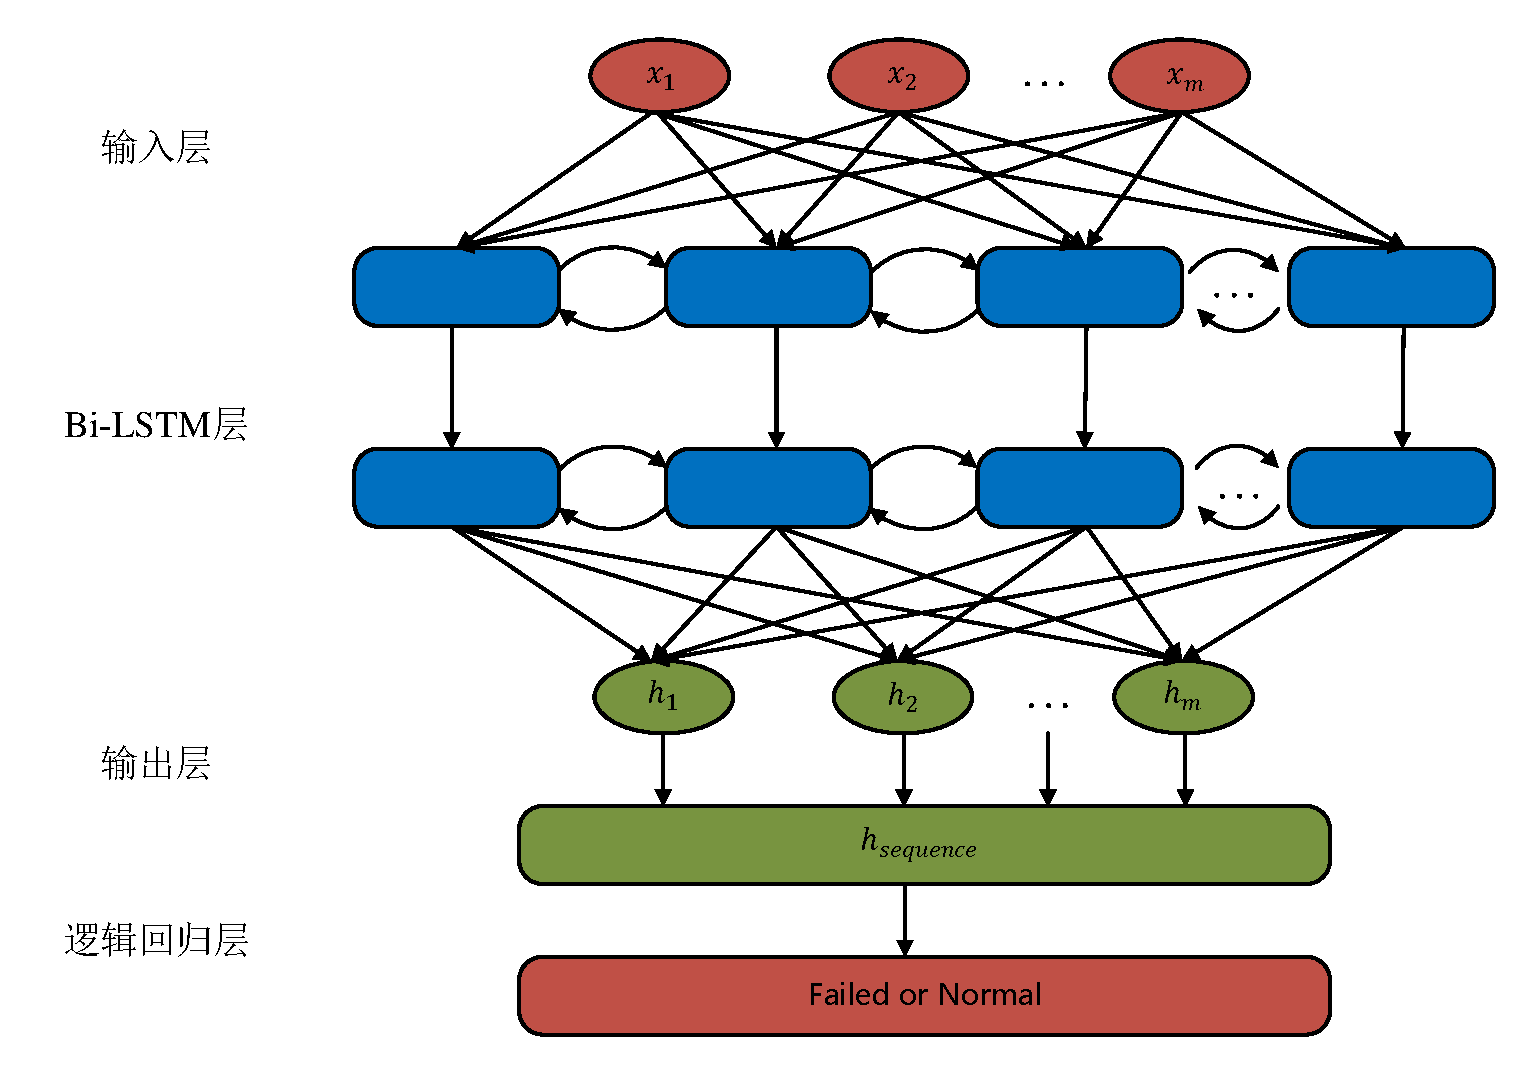
\includegraphics[width=.7\textwidth]{bilstm-model.pdf}
    \caption{基于双向长短期记忆神经网络的故障预测模型\label{bilstm-model}}
\end{figure}
图\ref{bilstm-model}所示为文献\parencite{gao2020task}用于故障预测的模型架构,可见其包含输入层、BiLSTM层、输出层和逻辑回归层。

输入层主要是数据的嵌入层。文献\parencite{gao2020task}拼接了同一时间点的CPU使用率、内存使用率、未映射页缓存、平均磁盘I/O时间、磁盘使用率、任务优先级、提交时间和提交次数共计8个特征。这样之后每个时间点都是一个8维的嵌入向量。
\begin{figure}[htbp]
    \centering
    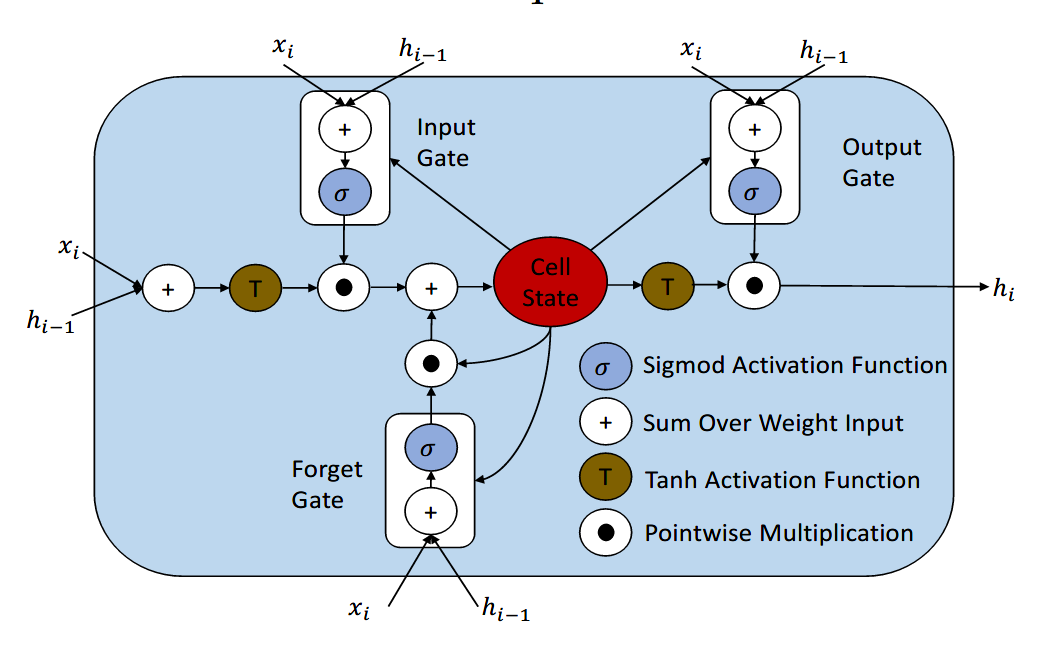
\includegraphics[width=.6\textwidth]{lstm-cell.png}
    \caption{双向长短期记忆网络神经单元\label{lstm-cell}}
\end{figure}

BiLSTM层完成了对时序数据的特征编码。该层会将输入的时序数据分别进行前向编码和后向编码,再将得到的前向隐状态和后向隐状态拼接得到最终的隐状态。经过上述步骤后,每个时间点的隐状态都会得到正向反向的上下文信息。图\ref{lstm-cell}展示了LSTM神经元内部的结构,可见其主要利用了非线性函数选择数据保存还是舍弃。具体实现上,每个神经元内部共有三个门控制其状态,包括输入门、遗忘门和输出门。输入门决定了应该更新哪个神经元状态,遗忘门决定了应该忽视掉什么信息,输出门决定输出隐状态的哪部分信息。该过程可以用公式\ref{lstm-cell-equation}表示:
\begin{equation}
    \begin{array}{l}
    g_{i}=\varphi\left(w_{g x} x_{i}+w_{g h} h_{i - 1}+b_{g}\right) \\
    n_{i}=\sigma\left(w_{n x} x_{i}+w_{n h} h_{i- 1}+b_{n}\right) \\
    f_{i}=\sigma\left(w_{f x} x_{i}+w_{f h} h_{i- 1}+b_{f}\right) \\
    o_{i}=\sigma\left(w_{o x} x_{i}+w_{o h} h_{i- 1}+b_{o}\right) \\
    s_{i}=g_{i} \odot n_{i}+s_{i -1} \odot f_{i} \\
    h_{i}=\varphi\left(s_{i}\right) \odot o_{i}
    \end{array}
    \label{lstm-cell-equation}
\end{equation}
其中$w_{gx}, w_{nx}, w_{fx} $和$w_{ox} $是记忆单元输入$x_{i}$的权重系数。$w_{gh}, w_{nh}, w_{fh} $和$w_{oh} $是记忆单元上一步输出$h_{i-1}$的权重系数。$b_{g}, b_{n}, b_{f},$ 和 $b_{o}$分别为输入信息$g_{i}$、输入门$n_{i}$、遗忘门$f_{i}$和输出门$o_{i}$对应的偏置系数。而$s_{i}$和$s_{i-1}$则分别为时间$i$和$i-1$的神经元状态。另外,$\odot$代表点乘,$\sigma$代表sigmoid激活函数,$\varphi$代表tanh激活函数。

输出层目的在于将输入序列中每个记忆单元隐状态整合起来。具体方式是将输入$X=\left\{x_{1}, x_{2} \ldots x_{m}\right\}$传入Bi-LSTM得到的表示序列$\left\{h_{1}, h_{2} \ldots h_{m}\right\}$进行式\ref{mean-pool}中所示的平均池化操作,得到序列表示向量$\widehat{h}$。
\begin{equation}
    \widehat{h}=\frac{1}{m} \sum_{i=1}^{m} h_{i}
    \label{mean-pool}
\end{equation}

逻辑回归层是预测当前数据序列将来是否会有故障的二分类层。具体实现上,该层将输出层得到的向量表示$\widehat{h}$输入$\operatorname{logstic}(.)$函数,计算会出现故障的概率。当概率大于阈值时,则预测会出现故障;反之,则预测不会出现故障。

\subsection{优化目标}
该模型的最终训练目标为正确分类每条数据序列。对应的损失函数为式\ref{memroy-net-loss}中所示。
\begin{equation}
    \mathcal{L}=-\sum_{i=1}^{n}\left[Y_{i} \log \left(f\left(X_{i} \right)\right)+\left(1-Y_{i}\right) \log \left(1-f\left(X_{i} \right)\right)\right]
    \label{memroy-net-loss}
\end{equation}

其中$X_{i}$表示第$i$条输入序列,$Y_{i}$为$X_{i}$对应的标签,即下一个时间点是否会有故障发生(1代表有故障发生,0代表不会有故障发生)。$f\left(.\right)$表示上文的BiLSTM模型。由损失函数计算得到损失值后,随机梯度下降会被用于更新模型参数。

\section{注意力机制}
注意力机制是一种自适应关注有效信息的机制,可以有效捕获长距离依赖信息\cite{mnih2014recurrent}。其本质上就是使用查询向量对一组键值向量计算权重分布,再根据权重分布对一组值向量加权平均。

注意力机制已经被广泛的应用在图像分类\cite{mnih2014recurrent}、神经机器翻译\cite{DBLP:conf/emnlp/LuongPM15}、多媒体推荐\cite{chen2017attentive}等领域。

在图像分类任务中,由于卷积神经网络的计算成本与输入图像的像素数成线性比例关系,因此在大图像上应用卷积神经网络的计算成本很高。为了解决巨大的计算成本问题,文献\parencite{mnih2014recurrent}提出了引入注意力机制的网络模型,所提出的模型自适应地从图像或视频中选择一系列区域,并且以高分辨率处理所选择的区域。

在机器翻译任务中,注意机制在翻译过程中有选择地聚焦于输入句子的有效部分,提高了机器翻译的准确性。Luong等人提出了两种机器翻译的注意机制方法:一种是始终关注所有源词的全局方法,另一种是只考虑源词子集的局部方法\cite{DBLP:conf/emnlp/LuongPM15}。

在多媒体推荐任务中,现有的协同过滤系统忽略了用户与多媒体内容间的隐含交互。文献\parencite{chen2017attentive}提出了两层注意机制来提取隐含交互。其中,底层自适应地选择组件级的隐含交互。上层自适应地选择项目级的隐含交互。两部分隐含交互会被结合起来输入经典的协同过滤模型。

\section{本章小结}
本章对本文中后续会涉及到的相关背景知识进行了介绍。本章首先介绍了支持向量机,支持向量机是进行分类的经典模型;其次介绍了关系图卷积神经网络,第四章会使用其获取实体上下文信息,实现组件-事件知识图谱实体的动态表示;随后介绍了双向长短期记忆神经网络,为第五章结合知识图谱和事件序列进行故障预测做了铺垫;最后介绍了注意力机制,第四章和第五章均使用其关注有效信息。